\section{Introduction}

\begin{mydef}
A sensor is a device that receives a stimulus
and responds with an electrical signal.
\end{mydef}

\begin{figure}[H]
    \centering
    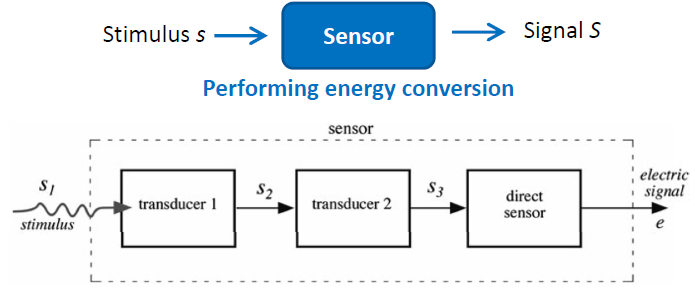
\includegraphics[width = 0.6\textwidth]{L1/img/sensor-def.PNG}
    \caption{A sensor may incorporate several transducers. $s_1, s_2$ and so on are various types of energy. Note that the last part is a direct sensor producing electrical output $e$.}
    \label{fig:sensor-def}
\end{figure}

\subsection{Sensor classification}

\subsubsection{Passive and active transducers}

\begin{mydef}
Stimulation of a \textbf{passive} transducer produces a
change in a passive electrical quantity ($R$, $L$, $C$) (e.g. thermistor, strain gauge).
\end{mydef}

\begin{mydef}
Stimulation of an \textbf{active} transducer generates a
voltage or current (generates electrical energy) (e.g. piezoelectric accelerometer, thermocouple).
\end{mydef}

\subsubsection{Absolute and relative sensors}

\begin{mydef}
An \textbf{absolute} sensor detects a stimulus in reference
to an absolute physical scale that is independent
of the measurement conditions (e.g. a thermistor).
\end{mydef}

\begin{mydef}
A \textbf{relative} sensor produces a signal that relates to
specific measurement conditions (e.g. a thermocouple).
A thermocouple output signal cannot be related to any particular 
temperature without referencing to a known baseline. 
\end{mydef}

Another example of the absolute and relative sensors is a pressure sensor. An absolute pressure sensor produces signal in reference to vacuum (absolute zero on a pressure scale). A relative pressure sensor produces signal with respect to a selected baseline that is not zero pressure (e.g. to the atmospheric pressure).
\vspace{0.3cm}

A photodiode is an \textbf{absolute active} sensor as the generated photocurrent varies with the absolute illumination level. 

\section{Characterization}

\subsection{Transfer function}

The transfer function gives a relation between the input and the output. It can be computed from:
\begin{itemize}
    \item  the mathematical model of the transduction mechanism,
    \item or the experimental characterization of the transduction (approximation of the transfer function).
\end{itemize}
The span refers to the sensor dynamic range: $DR = 20 \log_{10} \left( \frac{s2}{s1} \right)$ [dB].

\begin{figure}[H]
    \centering
    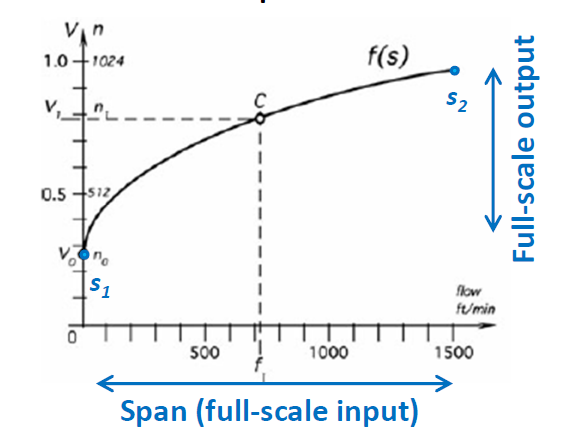
\includegraphics[width = 0.4\textwidth]{L1/img/trans-func.PNG}
    \caption{Transfer function}
    \label{fig:trans-func}
\end{figure}

A dynamic range of stimuli which may be converted by a sensor is called a span or an input full scale (FS). It represents the highest possible input value that can be applied to the sensor without causing an unacceptably large inaccuracy.


Full-scale output (FSO) is the algebraic difference between the electrical output signals measured with maximum input stimulus and the lowest input stimulus applied.

\subsubsection{Output format}
Different output signal types and data modulations can be observed:

\vspace{0.4cm}

\begin{minipage}[c]{.40\linewidth}	  
\begin{itemize}
    \item Signal type:
    \begin{itemize}
        \item voltage
        \item current
        \item charge
        \item digital code
    \end{itemize}
\end{itemize}
   \end{minipage} \hfill
   \begin{minipage}[c]{.52\linewidth}
   \begin{itemize}
    \item Data modulation
    \begin{itemize}
        \item DC
        \item amplitude, phase
        \item frequency
        \item duty-cycle
    \end{itemize}
\end{itemize}
   \end{minipage}
   
\subsubsection{Approximation of the transfer function}

\paragraph{Linear approximation}

$$ S = A + Bs $$

With $s$ the physical input stimulus (speed, pressure, temperature,...), $S$ the output signal, $A$ the intercept/\textbf{offset} (zero-crossing output signal) and $B$ the \textbf{sensitivity}/gain (slope).\textbf{ A and B are determined by calibration} (two parameters to determine).

When zero crossing is not possible (e.g. when $s$ is the temperature in K):

$$ S = S_0 + B(s-s_0) $$

\paragraph{Polynomial approximation}

Some sensors do not have a linear response. We can then use polynomial approximation to estimate their transfer function.

\begin{itemize}
    \item Second or third-order is usually enough for most sensor applications.
    \item Three or four parameters to determine by calibration.
\end{itemize}

\paragraph{Piecewise approximation}

\begin{itemize}
   \item Linear piecewise approximation is often adopted (continuous).
    \item Spline interpolation is used when continuous derivatives are required but at the expense of computational cost.
    \item The \textit{nodes} (or knots) need to be properly placed over the input span to minimize the error $\delta$ (nodes closer when the non linearity is high).
\end{itemize}

\begin{figure}[H]
    \centering
    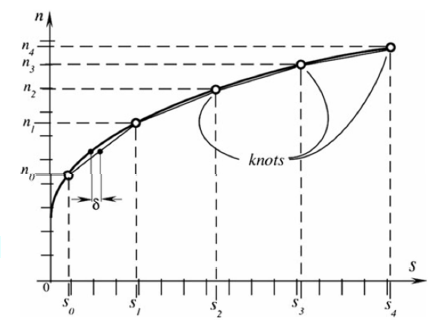
\includegraphics[width = 0.4\textwidth]{L1/img/piecewise.PNG}
    \caption{Linear piecewise approximation}
    \label{fig:piecewise}
\end{figure}

\subsection{Computation of stimulus}

There are three main ways to retrieve the input stimulus from the sensor output signal. 

\subsubsection{Inverting the transfer function}

Computation of the input stimulus from the output signal by inverting the transfer function.
This consists in analytically inverting the mathematical model. Given that most sensors have 
a non-linear transfer function, the computations needed for the reciprocal are often too heavy 
for microcontrollers (logarithm, exponential, fraction, \dots).

\begin{itemize}
    \item Low memory space required (only the transfer function coefficients are stored)
    \item Computation depends on the model type
    \item Accuracy depends on the model accuracy
    \item Heavy computation
on a microcontroller
for non linear transfer functions
\end{itemize}

\subsubsection{Use linear piecewise approximation (LPA)}

Using a simple mapping of the nodes present on the transfer function, the microcontroller determines 
on which interval the measured data is located, and applies a simple rule of three.

\begin{itemize}
    \item Light computation
    \item Scalable memory space requirement (only the node positions are stored)
    \item Trade-off between memory space and accuracy
\end{itemize}

\subsubsection{Iterative computation}

After a first guess of the solution $s_0$, a new value $s_{i+1}$ is determined 
following the Newton-Raphson's formula: 
$$s_{i+1} = s_{i} - \frac{f(s_i)-S_i}{f'(s_i)}$$
with $S$ the sensor signal output. When the absolute value between two guesses goes below a certain threshold, the last guess is taken as the solution.

\begin{itemize}
    \item Low to mid computation
    \item High memory space required
    \item High accuracy
\end{itemize}

\subsection{Non-idealities}

\subsubsection{Sensor (in)accuracy}

\begin{figure}[H]
    \centering
    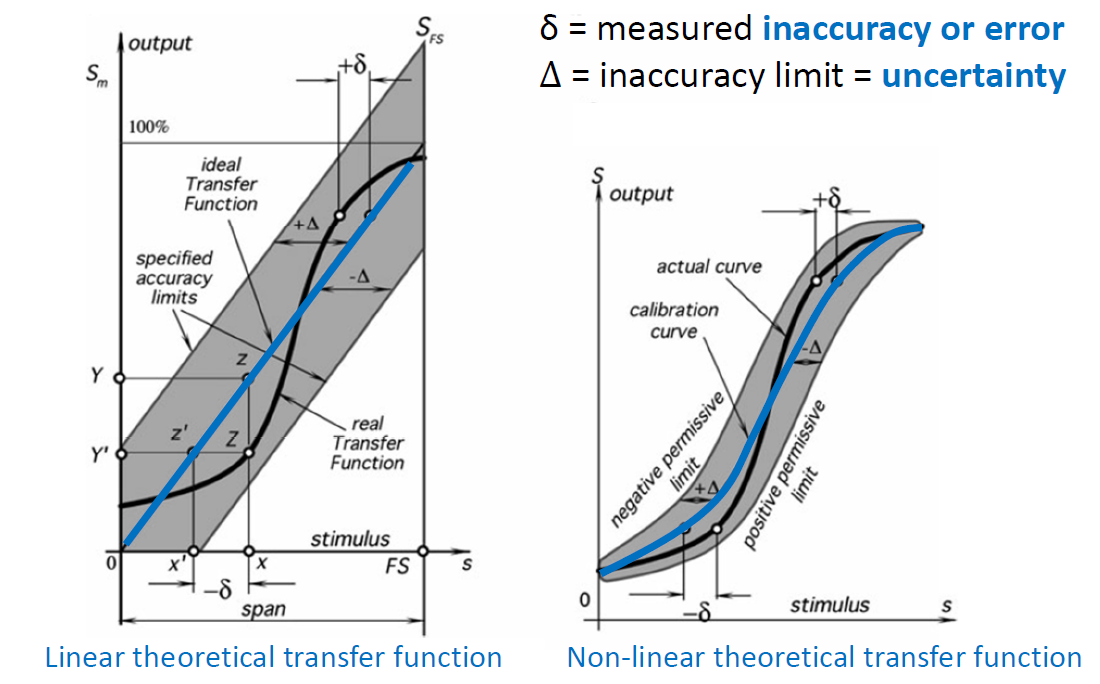
\includegraphics[width = 0.8\textwidth]{L1/img/inaccuracy.PNG}
    \caption{Linear piecewise approximation}
    \label{fig:innacuracy}
\end{figure}


Inaccuracy is measured as the highest deviation of a value represented by the sensor from the 
ideal or true value at its input. There are three categories of inaccuracy :

\begin{itemize}
    \item \textbf{Systematic} for all sensors
that leads to an approximate transfer function
    \item \textbf{Stochastic} from one fabricated
sensor to another (different readings on different sensors in the same conditions)
    \item \textbf{Stochastic in time} due to the noise (with a single senor)
\end{itemize}
These inaccuracies can be expressed in terms of :

\begin{itemize}
    \item Absolute input value $\rightarrow$ used when error is independent
from the input stimulus
    \item \% of the input span (full scale) $\rightarrow$ linear TF
    \item \% of the measured stimuli $\rightarrow$ non-linear TF
    \item Absolute output signal $\rightarrow$ Least-significant bits LSB
(considers quantization)
\end{itemize}
\textbf{Uncertainty} is comprised of all distorting effects, both systematic and random,
and is not limited to the inaccuracy of a transfer function.


\subsubsection{Modeling inaccuracies}

\begin{minipage}[c]{.45\linewidth}	  
The inaccuracy of a
sensor with a linear
transfer function is
usually expressed
in terms of:

\begin{itemize}
    \item Intercept/\textbf{offset} error: $ \delta_a = a_1 - a = \frac{s_1}{s_2 - s_1} \Delta $
    \item Sensitivity/\textbf{gain} error: $ \delta_b = - \frac{\Delta}{s_2 - s_1} $
\end{itemize}

\end{minipage} \hfill
\begin{minipage}[c]{.45\linewidth}
   \begin{figure}[H]
    \centering
    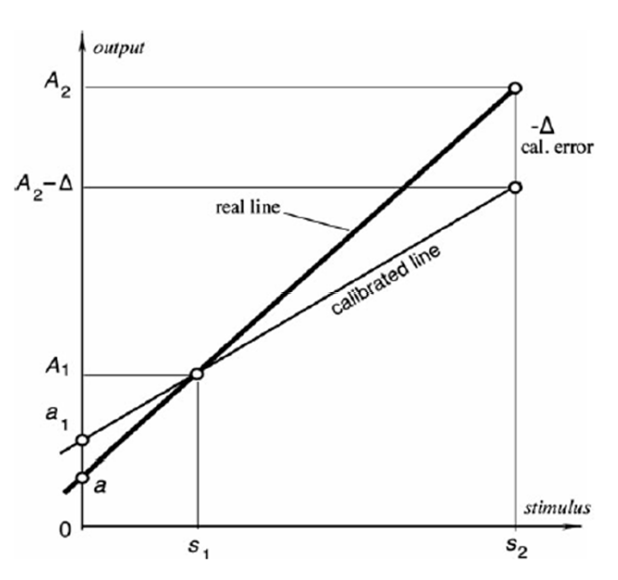
\includegraphics[width = 0.8\textwidth]{L1/img/calibration-error.PNG}
\end{figure}

   \end{minipage}

\subsubsection{Sources of inaccuracies}

\begin{itemize}
    \item Manufacturing tolerances
    \item Transducer / instrumentation impedance mismatch
    \item Parasitic components ($R$, $L$, $C$)
    \item Calibration error
    \item Intrinsic electrical noise of the transducer and the
instrumentation
    \item Environmental factors
    \begin{itemize}
        \item Electromagnetic interferences (EMI)
        \item Temperature/pressure/humidity variations
        \item Supply voltage
        \item HW stuff: moving cables, poor soldering, …
    \end{itemize}
\end{itemize}

\textbf{Note :} a sensor with an offset error but low scatter is better than another one with scattered results around the correct average. An offset error is easy to fix.

\subsubsection{Hysteresis}

\begin{minipage}[c]{.45\linewidth}	  
A hysteresis error is a deviation of the output of the sensor at a specified point of the input signal when it is approached from the opposite directions.

Typical causes for hysteresis are friction and structural changes in the materials. It is a typical characteristics of mechanical sensors. 
\end{minipage} \hfill
\begin{minipage}[c]{.45\linewidth}
   \begin{figure}[H]
    \centering
    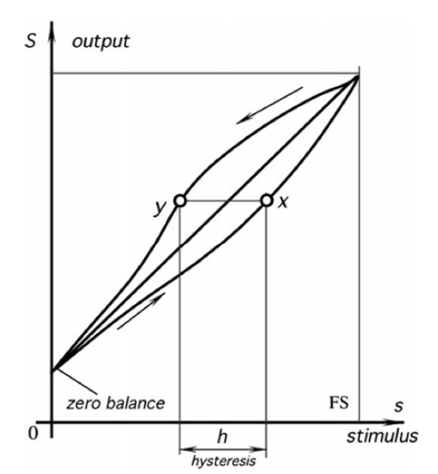
\includegraphics[width = 0.6\textwidth]{L1/img/hysteresis.PNG}
\end{figure}

   \end{minipage}
   

\subsubsection{Saturation and Dead-band}

\begin{minipage}[c]{.45\linewidth}	  
\textbf{Saturation} : When the sensor reaches
its operating limits (e.g. output voltage saturates at $V_{DD}$).
\begin{figure}[H]
    \centering
    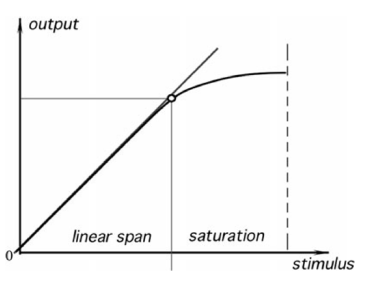
\includegraphics[width = 0.7\textwidth]{L1/img/sat.PNG}
\end{figure}
\end{minipage} \hfill
\begin{minipage}[c]{.45\linewidth}
\textbf{Dead-band} : Output signal stays at a
certain value (often zero) for a range of input stimuli
\begin{figure}[H]
    \centering
    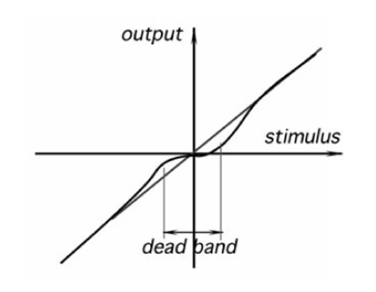
\includegraphics[width = 0.7\textwidth]{L1/img/dead-band.PNG}
\end{figure}
\end{minipage}
   
Both contribute to the non-linearity of the sensor if a linear transfer function is assumed !
   
\subsubsection{Output impedance}

The output impedance $Z_{out}$ is important to know to better interface a sensor with the electronic circuit.

   \begin{figure}[H]
    \centering
    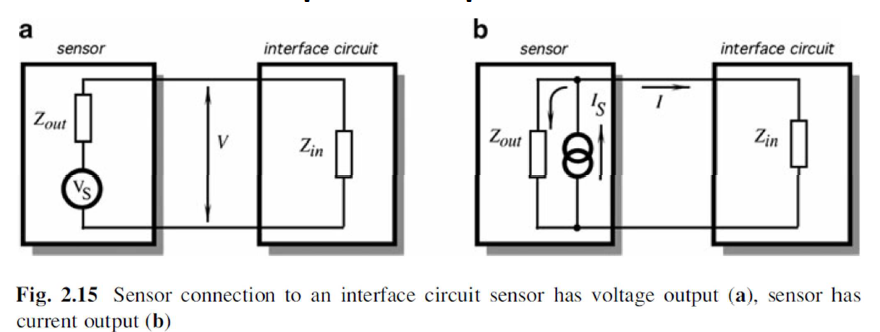
\includegraphics[width = 0.6\textwidth]{L1/img/output-impedance.PNG}
\end{figure}

\begin{itemize}
\item Output-voltage sensors require a low series $Z_{out}$ to have a small loss of voltage across it.
 \item Output-current sensors require a high parallel $Z_{out}$ to have a small current going in it.
 \item $Z_{out}$ may contain $R$, $L$, $C$ components.
 \item Parasitic RLC components on the sensor package, on
the board (PCB) contribute to $Z_{in}$ and $Z_{out}$.
\end{itemize}

\subsubsection{Resolution}

\begin{mydef}
Resolution is the smallest increment of stimulus which can be
sensed, so that it will induce a change of the output (even in no-noise condition).
\end{mydef}

It is typical of analog-to-digital conversion (ADC) (also in specific sensors e.g. infrared detectors
with grid distortion masks).

\subsubsection{Repeatability}

\begin{mydef}
The repeatability is the inability of a sensor to represent the same value
under presumably identical conditions (\textbf{short-term}).
\end{mydef}

\begin{minipage}{0.45 \linewidth}

\begin{itemize}
\item Usually expressed in \% of the full scale (FS), often
statistically extracted: $\sigma_s$/FS x 100\%
\item Causes: thermal noise, material plasticity, \dots
\item Long-term drift can also come from ageing effects
especially under stress conditions (high temperature,
high humidity, high $V_{DD}$, mechanical shocks, \dots)
\item Extreme cases of stress conditions can lead to
reliability issues by degrading the Mean-Time-To-Failure (MTTF)
\end{itemize}

\end{minipage}\hfill
\begin{minipage}{0.45 \linewidth}

\begin{figure}[H]
    \centering
    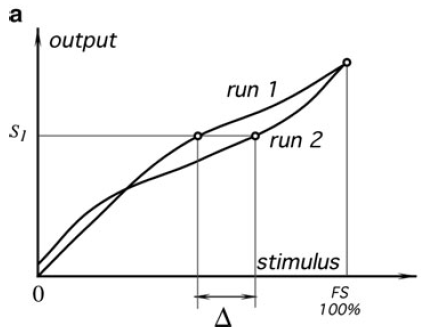
\includegraphics[width = 0.6\textwidth]{L1/img/repeatability.PNG}
    \caption{Repeatability error}
\end{figure}
\end{minipage}


\subsubsection{Dynamic characteristics}

When an input stimulus varies, a sensor response generally does not follow with perfect fidelity. The reason is that both the sensor and its coupling with the source of stimulus cannot always respond instantly. In other words, a sensor may be characterized with a time-dependent characteristic, which is called a dynamic characteristic.

For example, thermal sensors typically have a long “warm-up time” $\rightarrow$ slow response.
Dynamic characteristics can be classified by the order of the sensor:
\begin{itemize}
\item Zero-order: time-independent response $\rightarrow$ responds instantaneously
\item First-order: the relationship between $s(t)$ and $S(t)$ is
described by a first-order differential equation
\item Second-order: the relationship between $s(t)$ and $S(t)$ is
described by a second-order differential equation
\item \dots
\end{itemize}

\paragraph{First-order response}
Characterized by a cut-off frequency in the frequency domain
and a time constant in the time domain. Typical of sensors with one energy storage component
(e.g. a thermal capacity, an electrical capacitor, \dots).

\begin{figure}[H]
    \centering
    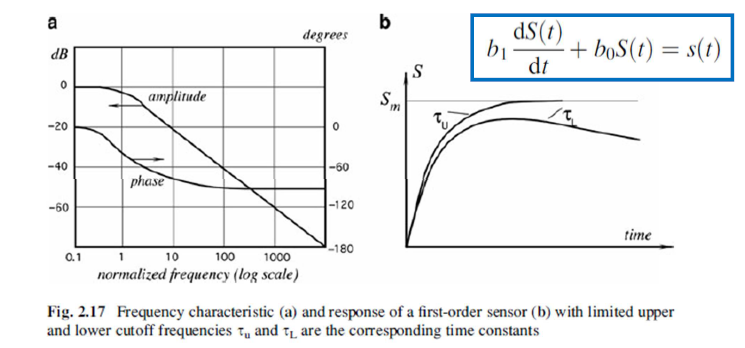
\includegraphics[width = 0.6\textwidth]{L1/img/first-order.PNG}
\end{figure}

\paragraph{Second-ordrer response}
Characterized by a resonant frequency in the frequency
domain and a periodic response in the time domain whose
duration depends on the damping factor. Typical of sensors with two energy storage components
(e.g. an accelerometer with an inertial mass and a spring).

\begin{figure}[H]
    \centering
    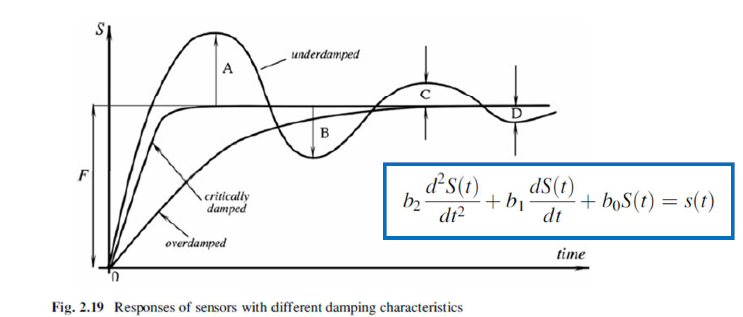
\includegraphics[width = 0.6\textwidth]{L1/img/second-order.PNG}
\end{figure}
